\chapter{ПРИМЕНЕНИЕ РЕГУЛЯРИЗАЦИИ НА ПРАКТИКЕ}

Описанная в \cite{turchin} и предыдущем разделе методика дает теоретический базис для решения многих задач анализа данных. Для практического применения необходимо также исследовать поведение результатов в зависимости от типа восстанавливаемой функции, а также от параметров алгебраизации и др. Сравнение работы метода при использовании различных базисов было проверено на нескольких модельных задачах. Для исследования работы метода заданная функция $\varphi$ свертывалась с интегральным ядром $K$, и к полученным значениям добавлялась случайная погрешность, имеющую нормальное распределение со средним равным нулю и шириной в 1\% от максимального значения функции на отрезке. Полученные данные обрабатывались описанным выше методом, реализующим аналитическое решение (\ref{eq:analit_solv}).


\section{Выбор параметра регуляризации}

При использовании статистического метода регуляризации удается последовательно получить распределение $P(\alpha | f)$, и вместо использования одного выбранного значение параметра регуляризации, можно произвести усреднение по всем возможным значениям параметра. Усреднение (интегрирование) производилось методом Монте-Карло с использованием метода существенной выборки. Однако, при достаточно узком распределении апостериорной вероятности $P(\alpha)$ интегрирование можно заменить нахождением наиболее вероятного $\alpha$, нахождением экстремума функции (\ref{eq:alphaaposter}) (Приложение \ref{sec:metod}). На Рис.\ref{pic:13} можно видеть, что оба метода дают схожий результат, однако при интегрировании уменьшаются погрешности найденного решения.

\begin{figure}[h! ]
	\label{pic:13}
	\center{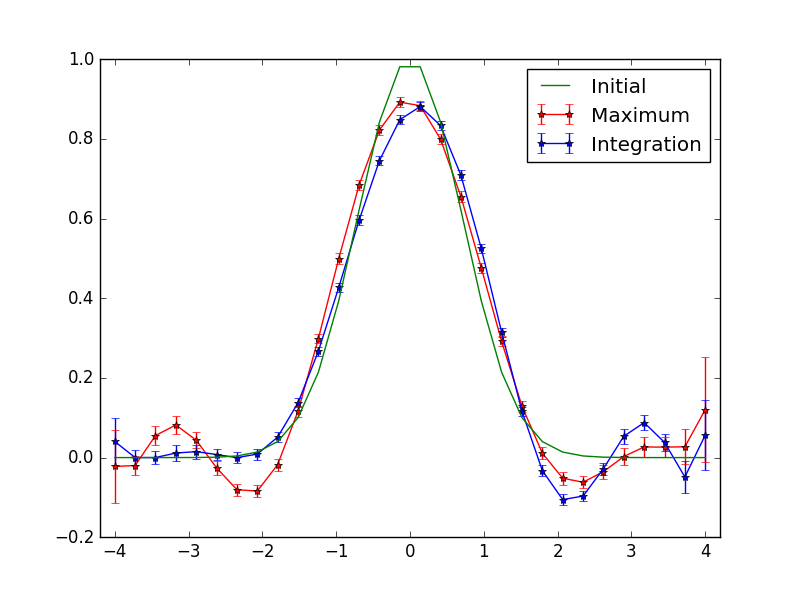
\includegraphics[scale=0.45]{integrate}}
	\caption{Результат восстановления функции с использованием усреднения по $\alpha$ (синяя кривая) и с поиском наиболее вероятного $\alpha$ (красная кривая).}
\end{figure}

\section{Базис алгебраизации}

Как было указано выше, метод регуляризации не ограничивает выбор конкретного базиса для разложения функций. В этом разделе будет представлено исследование зависимости результата регуляризации от выбора базиса. Описание математической процедуры алгебраизации уравнения (\ref{eq:opereq}) для разных базисов приведено в Приложении \ref{algebra}.

Ранее, в работе \cite{turovceva}, метод статистической регуляризации был реализован с использованием простейшего способа алгебраизации, в котором в качестве элементов $f_n$ использовались измеренные экспериментальные значения. В данной работе использовались три вида базисов: ряды Фурье, полиномы Лежандра и В-сплайны (описание базисов приведено в Приложениях \ref{sec:fourier}, \ref{sec:legendre} и \ref{sec:spline} соответственно). Сравнение работы метода при использовании различных базисов было проверено на нескольких модельных задачах.

Проведем сравнение восстановления функции с использованием разных базисов в условиях погрешностей эксперимента порядка 1\%. Для этого создадим для базисов равные условия --- одинаковую длину вектора $\phi$. Влияние величины погрешности на результат регуляризации будет рассмотрено в разделе ниже.

На рис.\ref{pic:gauss_3basis} представлено восстановление функции $\varphi(x)=e^{-x^2/2}$. Как можно увидеть из рис.\ref{pic:gauss_3basis}, метод успешно восстанавливает искомую функцию при использовании всех трех исследуемых базисов с незначительными различиями в результатах. 

На рис.\ref{pic:sigmoida_3basis} представлено восстановление сигмоиды $\varphi(x) = \frac{1}{1+e^{-x}}$. На примере этой функции становится заметна особенность базиса Фурье, а именно восприимчивость к асимптотике. При использовании базиса Фурье решение ``стремится'' быть симметричным на концах отрезка, что дает неправильное описание в случае асимметричной асимптотики. Это накладывает некоторые ограничения на использование того или иного базиса для исследования конкретной задачи.

\newpage
 \setlength{\textfloatsep}{10pt plus 1.0pt minus 2.0pt}
\setlength{\floatsep}{5pt plus 1.0pt minus 1.0pt}
\setlength{\intextsep}{5pt plus 1.0pt minus 1.0pt}

\begin{figure}[htbp! ]
	\center{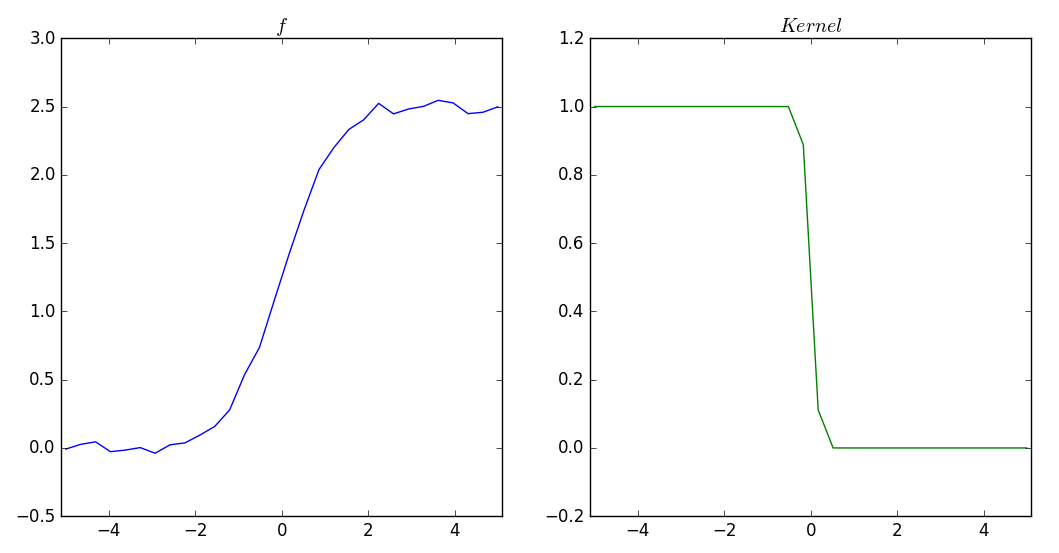
\includegraphics[width=0.7\linewidth]{new_figure_4} \\а)}
	\center{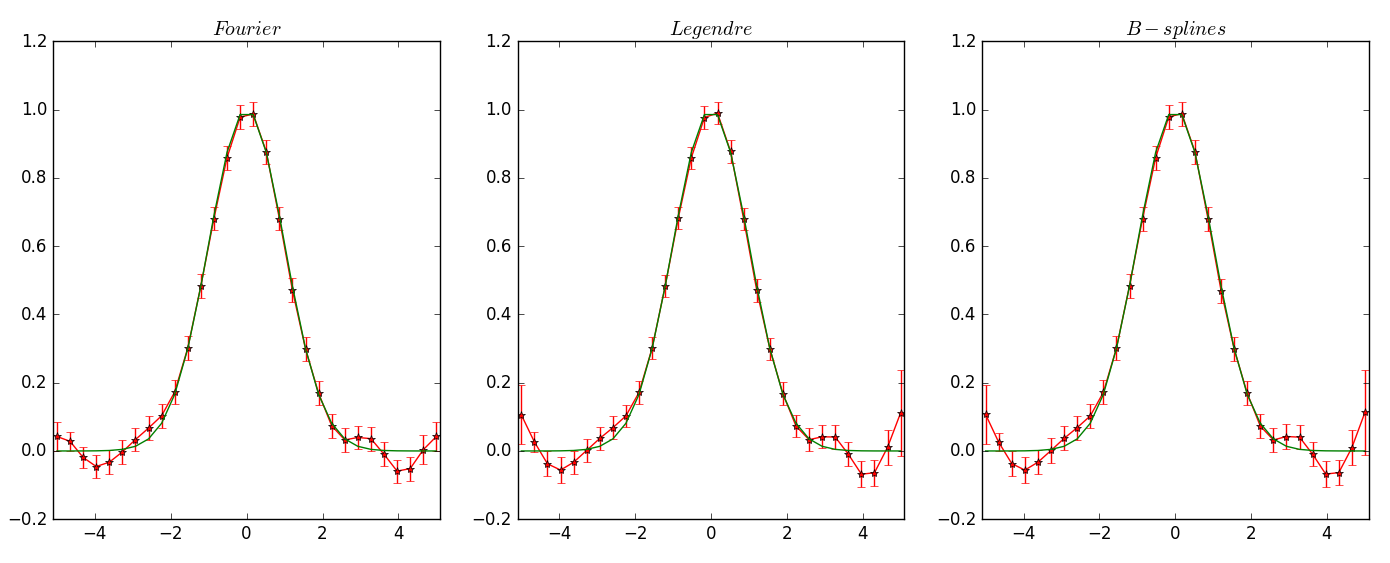
\includegraphics[width=1\linewidth]{new_figure_1} \\б)}
	\caption{Восстановление функции $e^{-x^2/2}$ со статистической погрешностью 1\%, 30 компонент, 30 узлов. Зеленая линия --- исходная функция, красная линия с точками --- результат регуляризации.}
	\label{pic:gauss_3basis}
\end{figure}

\begin{figure}[htbp! ]
	\center{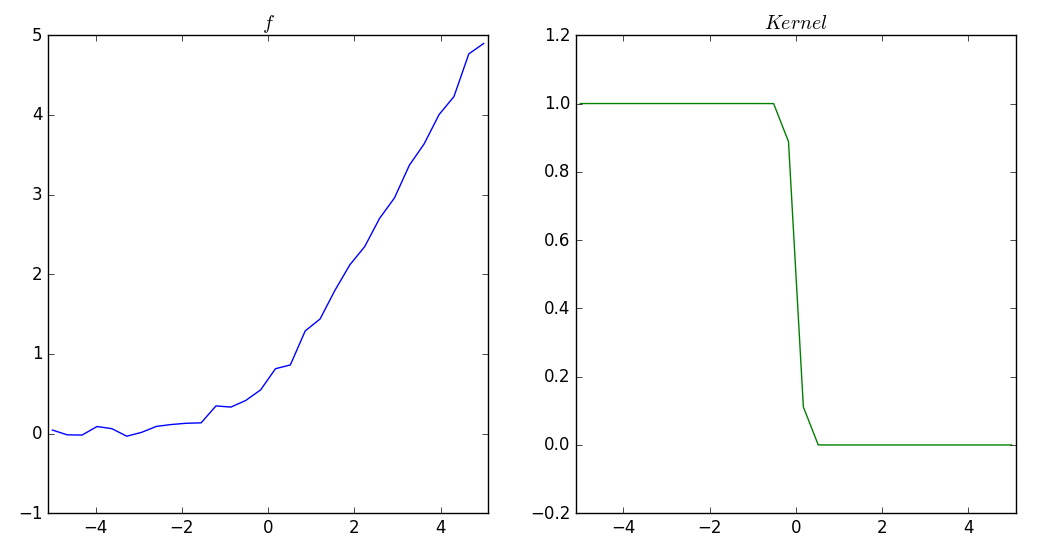
\includegraphics[width=0.8\linewidth]{new_figure_3} \put(0,0){a)}   }
	\center{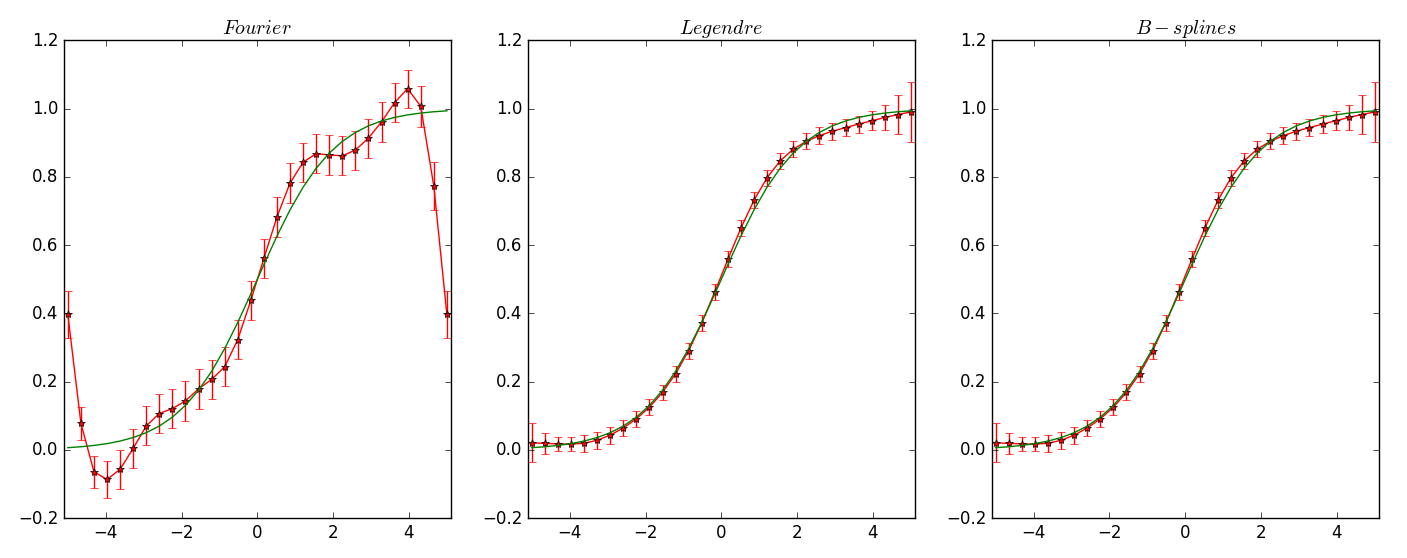
\includegraphics[width=1\linewidth]{new_figure_2} \\б)}
	\caption{Восстановление «сигмоиды» в трех базисах, малые погрешности (1\%) , 30 компонент, 30 узлов. Зеленая линия --- исходная функция, красная линия с точками --- результат регуляризации.}
	\label{pic:sigmoida_3basis}
\end{figure}
\newpage

\subsection{Количество базисных функций}

При задании базиса из полиномов Лежандра или компонент Фурье необходимо выбрать определенное число базисных функций. Рассмотрим влияние выбора этого числа для каждого из базисов. На Рис.\ref{pic:6} и Рис.\ref{pic:7} представлено восстановление функции Гаусса с помощью разного числа компонент в базисах полиномов Лежандра и рядов Фурье соответственно.

\begin{comment}
\begin{figure}[h! ]
	\label{pic:6}
	\center{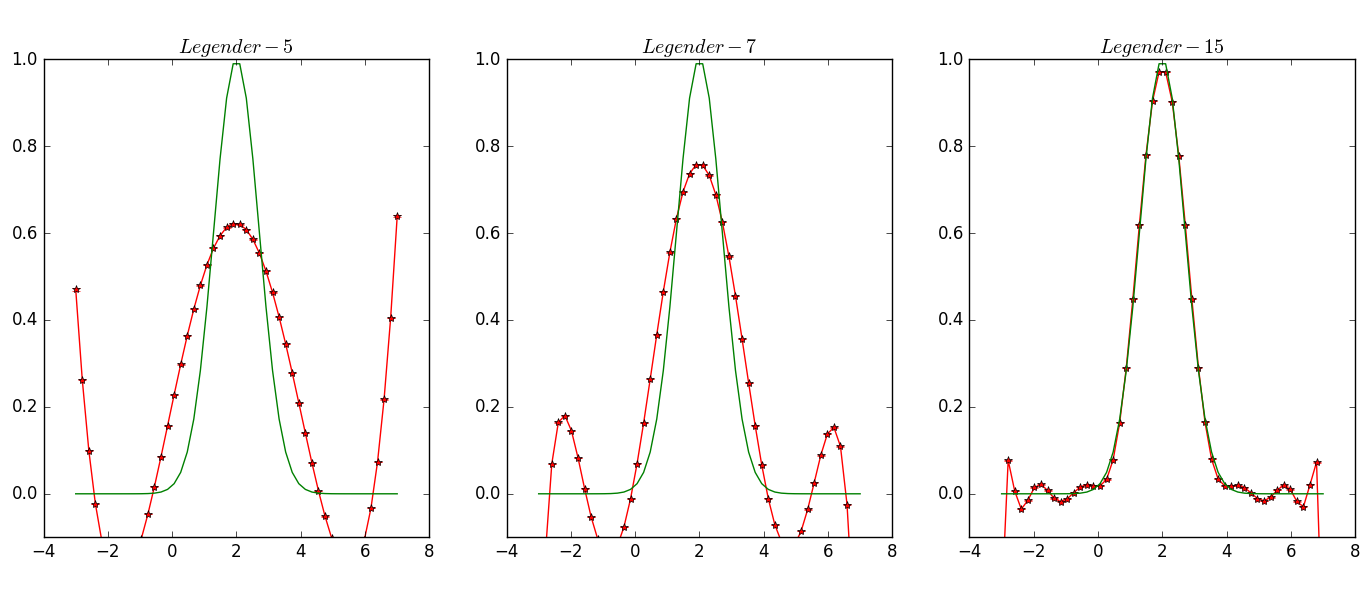
\includegraphics[width=1\linewidth]{pic6} }
	\caption{Восстановление функции Гаусса $e^{-(x-2)^2}$ с помощью 5, 7 и 15 полиномов Лежандра соответственно. Зеленая линия --- исходная функция, красная линия с точками --- результат восстановления.}
\end{figure}


\begin{figure}[h! ]
	\label{pic:7}
	\center{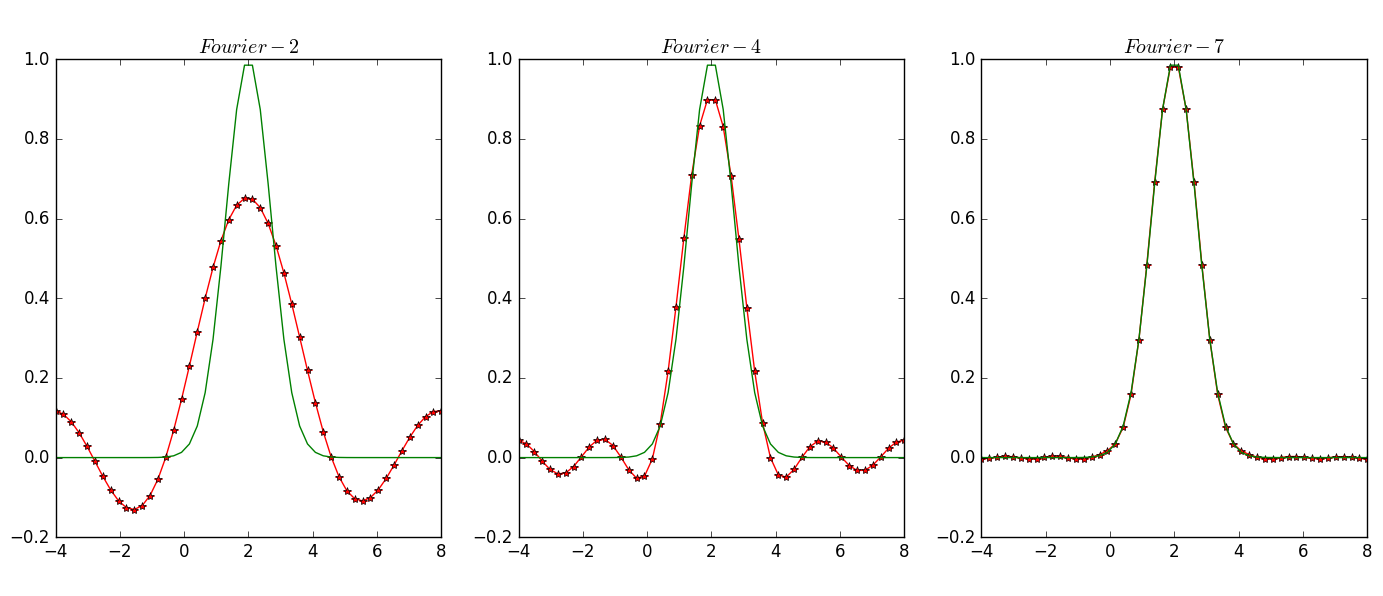
\includegraphics[width=1\linewidth]{pic7}}
	\caption{Восстановление функции Гаусса $e^{-(x-2)^2}$ с помощью 4, 8 и 14 компонент Фурье соответственно. Зеленая линия --- исходная функция, красная линия с точками --- результат восстановления.}
\end{figure}
\end{comment}

Как можно видеть, при использовании базиса полиномов Лежандра необходимо большее число компонент для получения хорошего описания, чем при использовании базиса Фурье. Следовательно при использовании полиномов Лежандра требуется больше вычислительного времени, что является особенностью данного базиса. На Рис.\ref{pic:graf1} представлены графики зависимостей среднего квадрата отклонения от исходной функции и средней погрешности решения от числа базисных компонент. Как видно из данных графиков, значение отклонения и погрешностей с ростом числа компонент выходит на константу, значит можно выбрать оптимальное число базисных компонент для восстановления, дальнейшее добавление базисных функций не будет значительно улучшать результат восстановления.
В целом, говоря о необходимом количестве базисных компонент, стоит заметить, что в методе происходит восстановление именно разложенной по базису функции. Следовательно, значительное влияние на результат имеет именно качество алгебраизации уравнения Фредгольма. 
\begin{comment}
\begin{figure}[h! ]
	\label{pic:7}
	\center{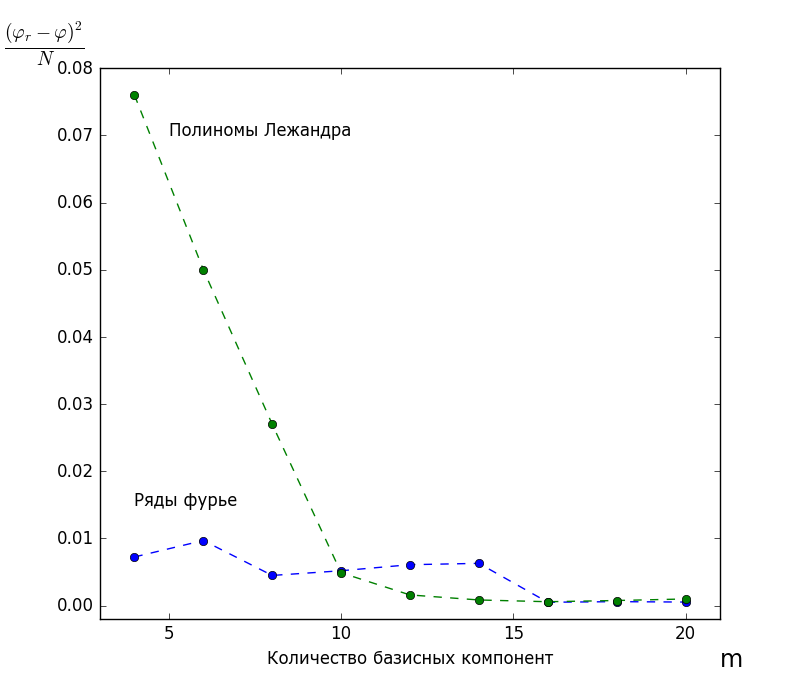
\includegraphics[width=0.9\linewidth]{legendre_and_fourier_components}}
	\caption{График для разных значений m для лежандров и фурье.}
\end{figure}
\end{comment}

\begin{figure}[h! ]
\begin{center}
\begin{minipage}[h]{0.48\linewidth}
	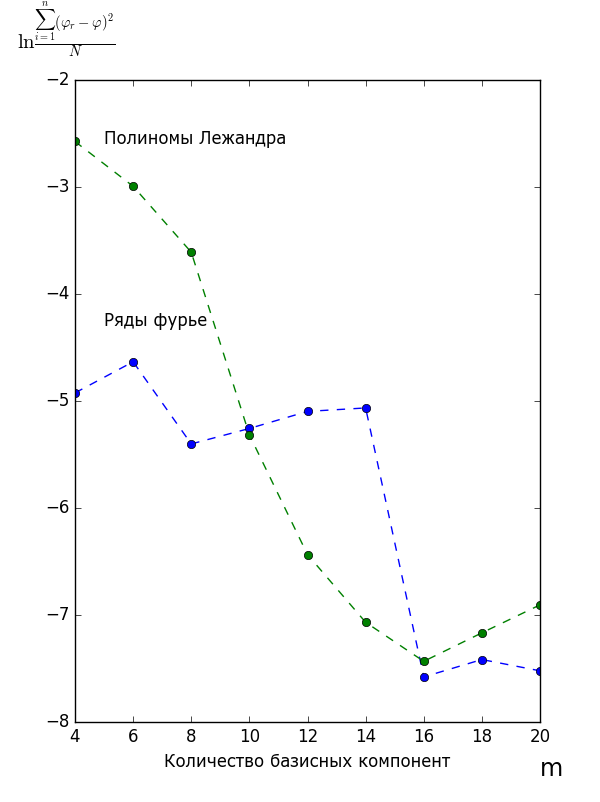
\includegraphics[width=0.9\linewidth]{log_legendre_and_fourier_components} \\а)
\end{minipage}
	\hfill
\begin{minipage}[h]{0.48\linewidth}
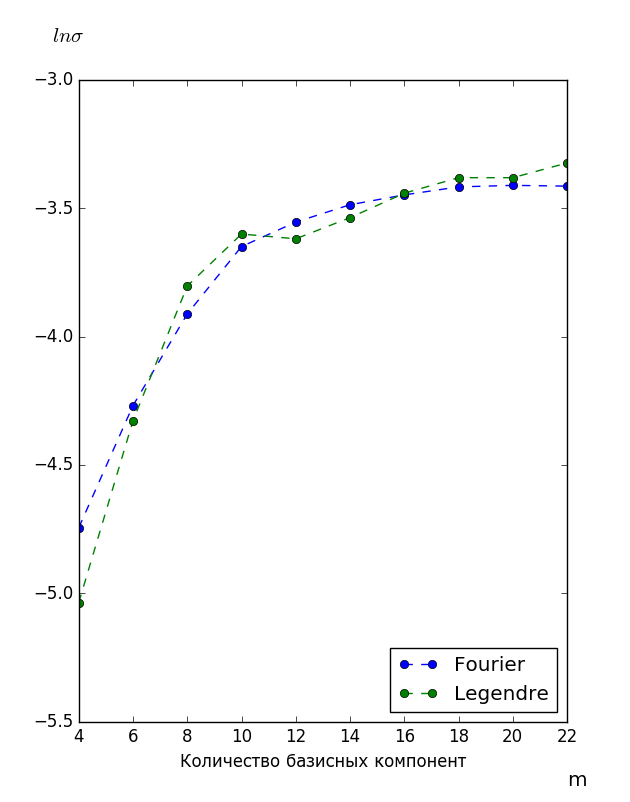
\includegraphics[width=0.9\linewidth]{log_sigma} \\б)
\end{minipage}
	\caption{а) Зависимость среднего квадрата отклонения от количества базисных компонент. б) Зависимость средней погрешности решения от количества базисных компонент}
\label{pic:graf1}
\end{center}
\end{figure}


\subsection{Количество экспериментальных точек и узлов сетки}

Изучим теперь свойства базиса B-сплайнов, зависящих от количества экспериментальных точек (узлов). Аналогично ситуации с числом базисных компонент, при увеличении числа узлов на отрезке средний квадрат отклонения от исходной функции выходит на константу (Рис.\ref{pic:graf2})
\begin{figure}[h! ]
	\label{pic:7}
	\center{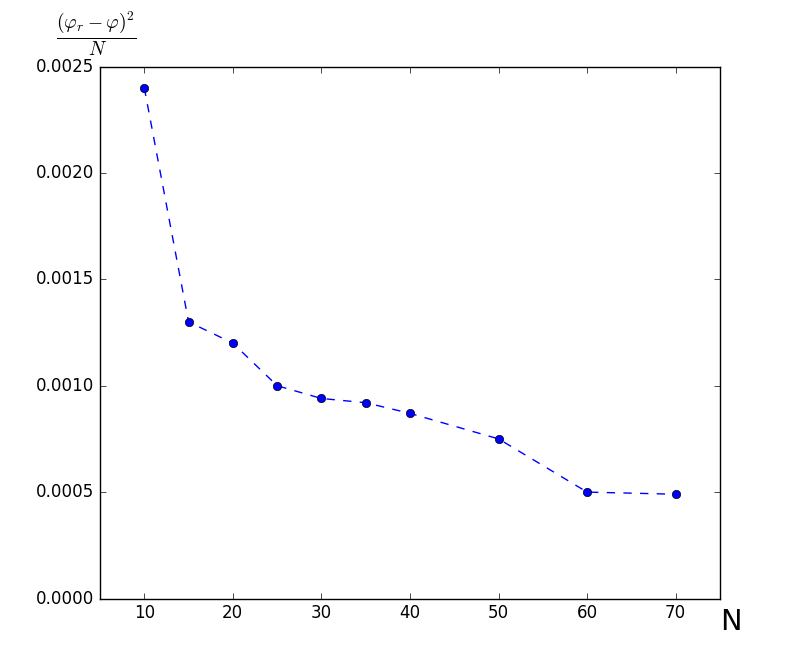
\includegraphics[width=0.75\linewidth]{splines_knots}}
	\caption{График зависимости среднего квадрата отклонения от числа узлов для В-сплайнов.}
	\label{pic:graf2}
\end{figure}


\section{Ядро}

Все случаи, рассмотренные выше, относились к восстановлению функций, свернутых с интегральным ядром. Теперь рассмотрим случай Гауссовского ядра $K=e^{-(x-2)^2}$ (Рис.\ref{pic:gausskernel}) Результат свертки данного ядра с исходной функцией Гаусса показан на Рис.\ref{pic:gausskernel}. Как можно увидеть, в случае неинтегрального ядра исходная функция также успешно восстановлена. Однако, как и в случае рассмотрения разных базисов, нельзя утверждать, что метод и выбранный базис универсален для всех типов ядер.

\begin{comment}
\begin{figure}[h! ]
\begin{center}
\begin{minipage}[h]{0.3\linewidth}
	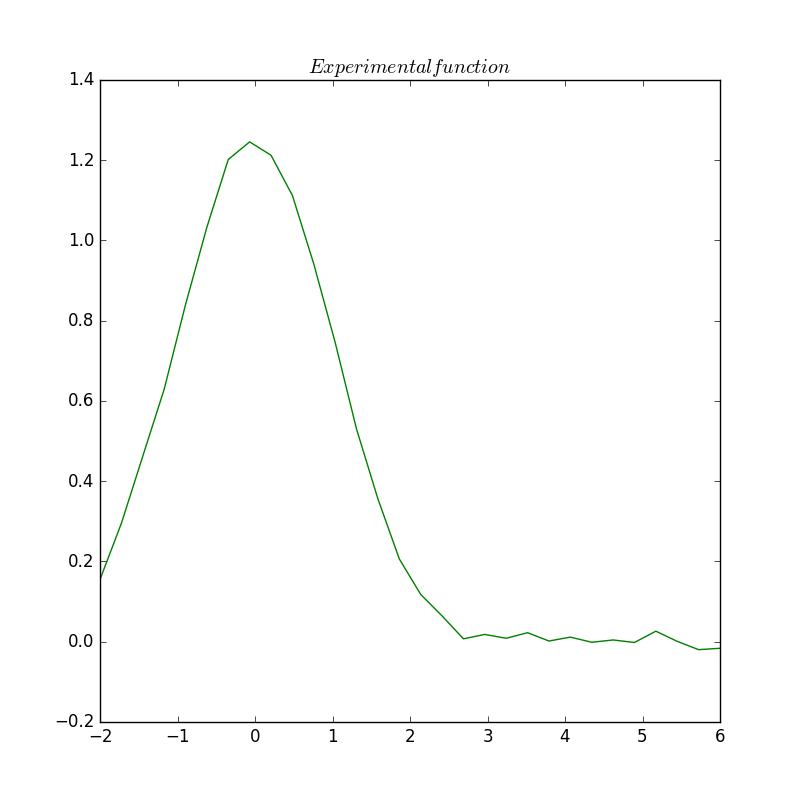
\includegraphics[width=1\linewidth]{func_10} \\а)
\end{minipage}
	\hfill
\begin{minipage}[h]{0.3\linewidth}
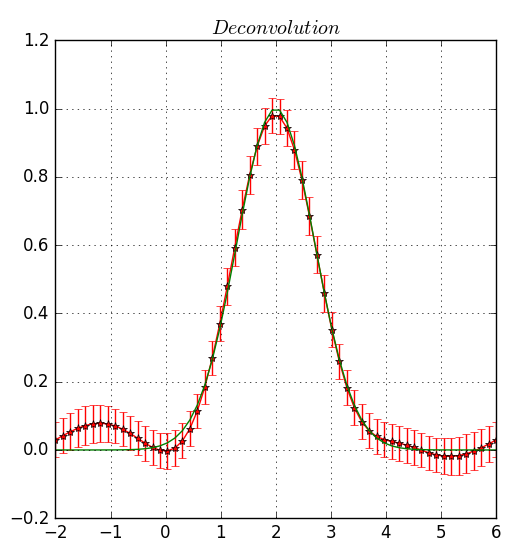
\includegraphics[width=1\linewidth]{pic10a} \\б)
\end{minipage}
\hfill
\begin{minipage}[h]{0.3\linewidth}
	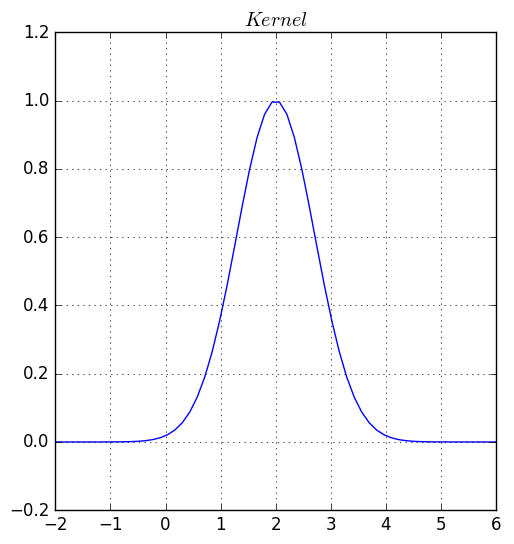
\includegraphics[width=1\linewidth]{pic10b} \\в)
\end{minipage}
	\caption{Случай неинтегрального ядра. а) Экспериментальные значения. б) Ядро $K=e^{-(x-2)^2}$. в) Результат восстановления с помощью базиса Фурье (20 компонент) со статистическими погрешностями 1\%, зеленая линия --- исходная функция, красная линия с точками --- результат регуляризации.}
\label{pic:gausskernel}
\end{center}
\end{figure}
\end{comment}
   
\section{Влияние погрешностей измерения}

Проанализируем влияние величины шумов при измерении на восстановление функции. Для определенности все операции будем проводить в базисе Фурье. На Рис.\ref{pic:noize}. представлено восстановление функции Гаусса в случае разных случайных погрешностей вплоть до 10\%. При восстановлении использовался базис Фурье.

Для успешной работы метода недопустимы нулевые случайные погрешности, так как это приведет к сингулярности при обращении матрицы $\Sigma$ (см. формулу (\ref{eq:gaussP})). Поэтому для моделирования случая с нулевыми шумами были использованы достаточно малые погрешности - 0.001\%. Восстановление в случае с нулевыми ошибками просто соответствует решению интегрального уравнения и восстановленное решение должно совпадать с исходной функцией.

Как можно видеть из Рис.\ref{pic:noize}, при малых статистических ошибках восстановленная кривая совпадает с исходной функцией, что полностью согласуется с ожиданием. Погрешности восстановления также очень малы.

\begin{comment}
\begin{figure}[h! ]
	\center{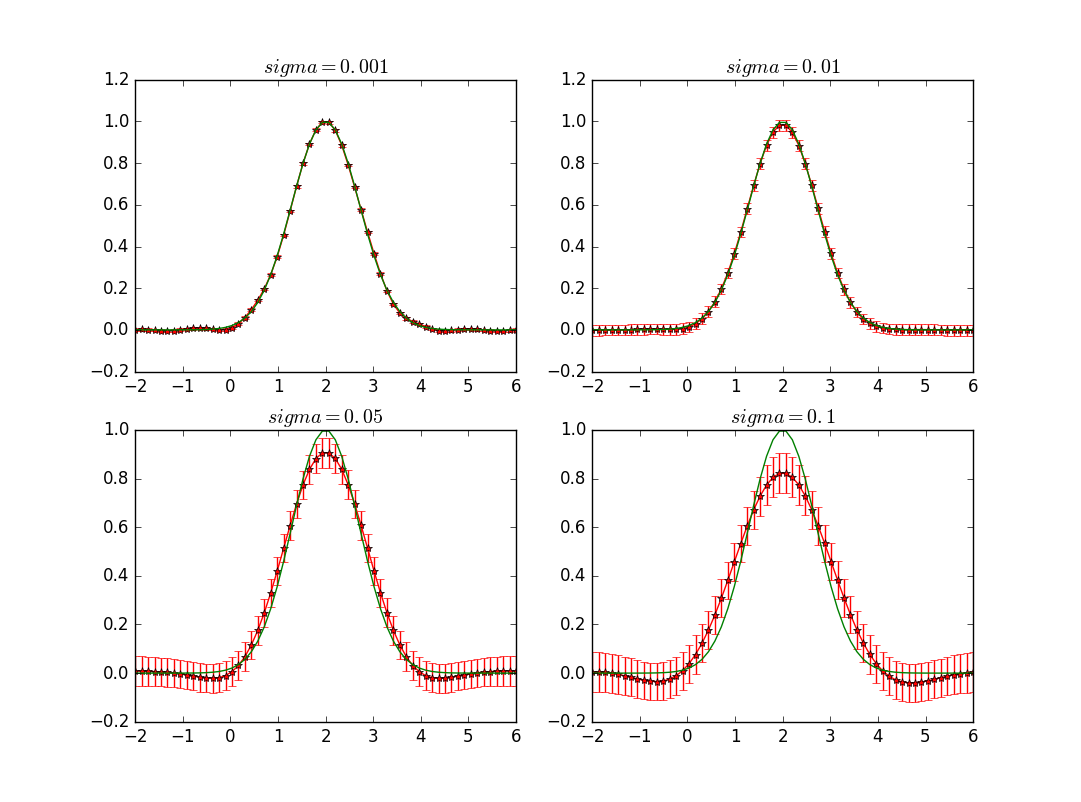
\includegraphics[scale=0.45]{pic12}}
	\caption{Восстановление гаусса с разными погрешностями при измерении: 0.001\%, 1\%, 5\% и 10\%. Зеленая линия --- исходная функция, красная линия с точками --- результат восстановления.}
	\label{pic:noize}
\end{figure}
\end{comment}

Увеличение случайных погрешностей при измерениях искажает решение, делая пик более сглаженным, а также приводит к увеличению погрешностей восстановления. Исходная и восстановленная кривая совпадают в пределах погрешностей восстановления при величине ошибок меньше 5\%. Еще одно следствие увеличения случайных погрешностей - возникновение и рост ложных осцилляций на краях (раскачивания). Раскачивания присутствуют в результатах восстановления с использованием любого базиса. Раскачивание на краях можно устранить, введя дополнительную априорную информацию о граничных услвоиях. Исследование граничных условий выходит за рамки этой работы.

%%

\section{Введение дополнительной априорной информации}

Отличием статистического метода от классических является возможность введения дополнительной априорной информации об исходной функции. Рассмотрим случай, когда кроме гладкости функции также известно, что функция неотрицательна. Такое условие можно учесть, домножив апостериорную плотность вероятности на дополнительное распределение по $\varphi$:
\begin{equation}
    P'(\vec{\varphi}|\vec{f}) \sim \zeta(\vec{\varphi})P(\vec{\varphi}|\vec{f}), ~\zeta(\vec{\varphi})=0,  F_i(\vec{\varphi})>0. 
\end{equation}

Нахождение наилучшего решения с таким условием сводится к задаче оптимизации уже найденного решения с учетом неотрицательности результирующей функции во всех точках. Подобный метод был описан в работе \cite{turovceva}. Программные методы оптимизации также позволяют определять условия в виде равенств, тогда кроме неотрицательности в точках можно добавить, к примеру, уcловия равенcтва нулю функции на концах отрезка. Как можно видеть из Рис.\ref{pic:aprioriopt}, введение дополнительной априорной информации значительно улучшило восстановление.

\begin{comment}
\begin{figure}[h!]
\begin{center}
\begin{minipage}[h]{0.45\linewidth}
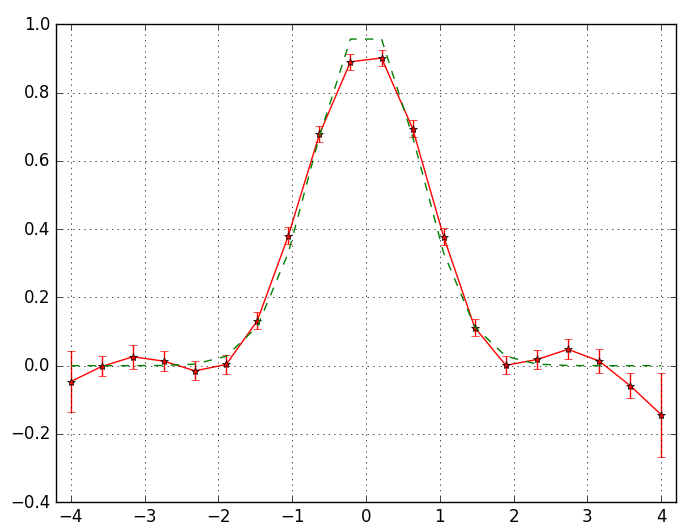
\includegraphics[width=1\linewidth]{no-negative1} \\а)
\end{minipage}
\hfill 
\begin{minipage}[h]{0.45\linewidth}
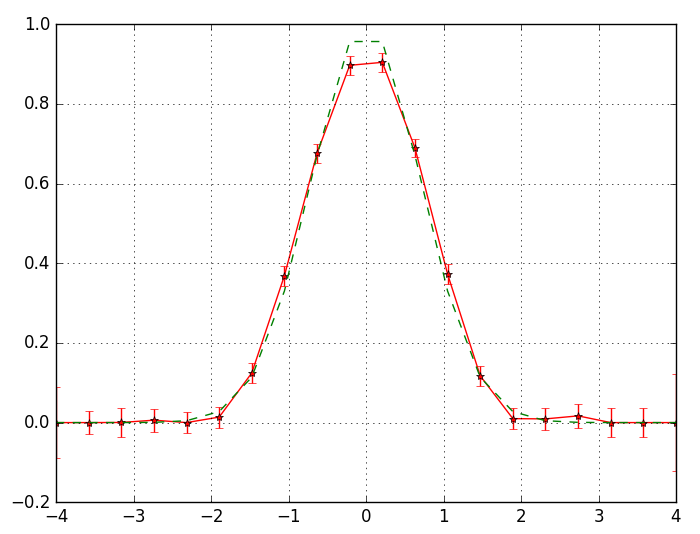
\includegraphics[width=1\linewidth]{no-negative2} \\б)
    \end{minipage}
    \caption{а) Результат регуляризации до добавления дополнительной информации. б) Результат оптимизации решения. Зеленая линия --- исходная функция, красная линия с точками --- результат регуляризации.}
\end{center}
\end{figure}
\end{comment}

\section{Исследование метода на примере данных эксперимента Troitsk nu-mass}
Рассмотрим работу метода в условиях обработки даных с реального физического эксперимента. Для проверки результата регуляризации были использованы данные измерения дифференциального сечения рассеяния электронов на изотопах водорода, полученные в эксперименте Troitsk nu-mass в 2015 году. Постановка задачи такая же: искомый спектр рассеянных элекронов сворачивается с известной разрешающей функцией спектрометра. В работе \cite{numass} приведены результаты обработки этих данных при помощи фитирования сложной функцией. Такой подход имеет два существенных недостатка:
\begin{enumerate}
    \item Функция, которой осуществляется фитирование подбирается ``на глаз'' и не имеет никакого физического обоснования. В частности таким образом невозможно исследовать особенности изучаемой функции, не заложенные в исходную модель.
    \item Имеют место сильные корреляции между параметрами фитирующей функции, которые сильно затрудняют фитирование, в некоторых случаях делая его невозможным.
\end{enumerate}
На Рис.\ref{pic:exp1} представлены экспериментальные данные - интегральный спектр рассеянных электронов. На Рис.\ref{pic:exp2} показаны результат регуляризации и результат фитирования. Регуляризация производилась с использованием базиса B-сплайнов с добавлением нулевых граничных условий. Как можно видеть, результат регуляризации хорошо согласуется с полученным ранее, однако можно еще улучшить результат, если добавить дополнительное условие неотрицательности функции, а также учесть влияние фона (площадка слева на экспериментальных данных Рис.\ref{pic:exp1}).